\documentclass[10pt]{standalone}

%% For sans serfen Schrift:
%\usepackage[onehalfspacing]{setspace}
%\usepackage{helvet}
%\renewcommand{\familydefault}{\sfdefault}


\usepackage[utf8]{inputenc}
\usepackage[german]{babel}
\usepackage[T1]{fontenc}
\usepackage{graphicx}
\usepackage{lmodern}

\usepackage{amsmath}
\usepackage{amsfonts}
\usepackage{amssymb}
\usepackage{gensymb}
\usepackage{bm}
\usepackage{ifthen}
\usepackage{array}
\usepackage{eurosym}

\usepackage{tikz}
\usetikzlibrary{calc,patterns,
                 decorations.pathmorphing,
                 decorations.markings,
                 decorations.pathreplacing}
\usetikzlibrary{trees,arrows, scopes}
\usetikzlibrary{shapes}
\usetikzlibrary{positioning}
\usetikzlibrary{fadings}
\usepackage{tikz-3dplot}
\usetikzlibrary{matrix,fit, backgrounds}


\usepackage{pgfplots}
\usepgfplotslibrary{groupplots}
\pgfplotsset{compat=newest}

                 
\newcommand*\circled[1]{\tikz[baseline=(char.base)]{
            \node[shape=circle,draw,inner sep=2pt,solid,fill=white] (char) {#1};}}
            
            
            
\usetikzlibrary{patterns}

\pgfdeclarepatternformonly[\LineSpace]{my north east lines}{\pgfqpoint{-1pt}{-1pt}}{\pgfqpoint{\LineSpace}{\LineSpace}}{\pgfqpoint{\LineSpace}{\LineSpace}}%
{
    \pgfsetlinewidth{0.4pt}
    \pgfpathmoveto{\pgfqpoint{0pt}{0pt}}
    \pgfpathlineto{\pgfqpoint{\LineSpace + 0.1pt}{\LineSpace + 0.1pt}}
    \pgfusepath{stroke}
}


\pgfdeclarepatternformonly[\LineSpace]{my north west lines}{\pgfqpoint{-1pt}{-1pt}}{\pgfqpoint{\LineSpace}{\LineSpace}}{\pgfqpoint{\LineSpace}{\LineSpace}}%
{
    \pgfsetlinewidth{0.4pt}
    \pgfpathmoveto{\pgfqpoint{0pt}{\LineSpace}}
    \pgfpathlineto{\pgfqpoint{\LineSpace + 0.1pt}{-0.1pt}}
    \pgfusepath{stroke}
}

\newdimen\LineSpace
\tikzset{
    line space/.code={\LineSpace=#1},
    line space=3pt
}

\newcommand\centerofmass{%
    \tikz[radius=0.4em] {%
        \fill (0,0) -- ++(0.4em,0) arc [start angle=0,end angle=90] -- ++(0,-0.8em) arc [start angle=270, end angle=180];%
        \draw (0,0) circle;%
    }%
}



\begin{document}
\begin{tikzpicture}[
schnitt/.style={decoration = {zigzag,segment length = 15mm, amplitude = 1mm}, decorate},
kontur/.style={thick},
top/.style={line width=1mm},
forceattack/.style={very thick, -latex},
frame/.style={line width=1.5mm, gray!50, opacity=.5, rounded corners=.2cm}
]

\path[clip](-7.1,-.7)rectangle(7,4.1);


\path (0,.1)node[above left]{
	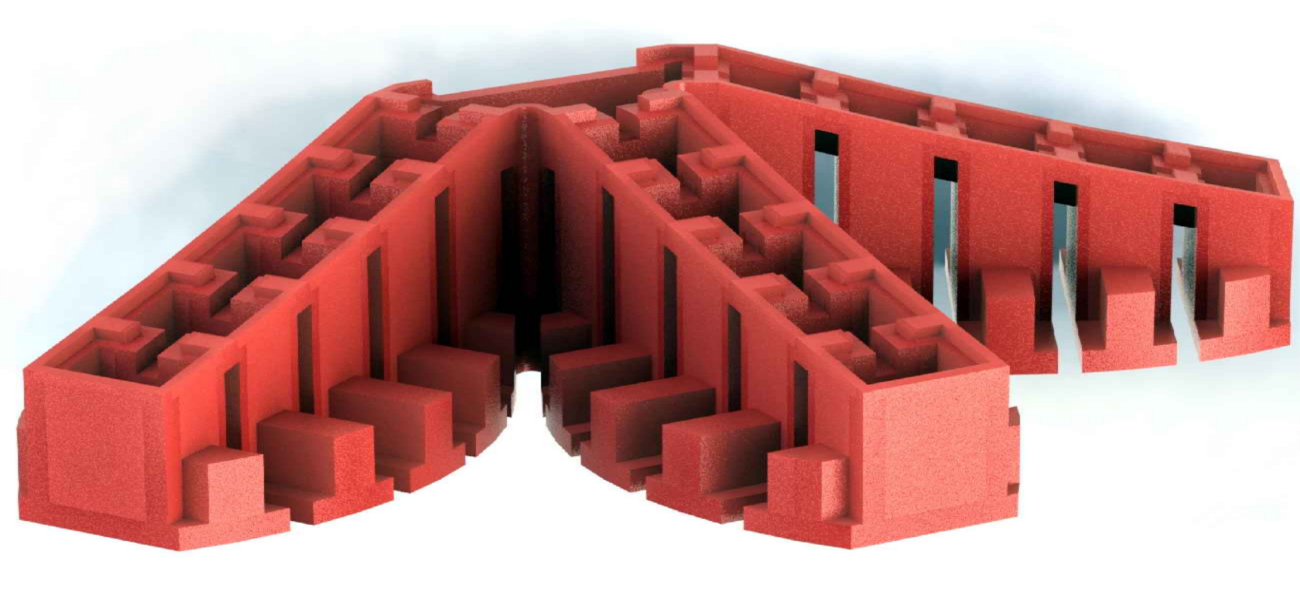
\includegraphics[width=7cm]{render.png}};

%% GRID
% \draw[help lines] (0,0)grid(-7,4);



%%% Sigma
\def\start{-1.6} \def\ende{-.25} \def\step{.2} \def\y{.85}
\draw (\start,\y)--(\ende,\y)node[midway, below]{$\sigma$};
\pgfmathsetmacro{\second}{\start+\step}
\foreach \x in {\start, \second, ..., \ende}{
	\draw[-latex] (\x+.15,\y)--++(0,.3);
}

\draw (-4.3,.7)coordinate(start)--(-2.3,-.5)coordinate(ende)node[midway, below]{$\sigma$};
\def\N{10}
\foreach \n in {0,1,...,\N}{
	\pgfmathsetmacro{\pos}{\n/\N}
	\path (start)--(ende)coordinate[pos=\pos](X);
	\draw[-latex] (X)--++(0,.3);
}


%%% Freikoerperbild

% Rahmen
\def\rx{6.5}
\def\rc{.8}
\draw[frame] (-1.05,2.07)coordinate(C)circle(\rc);
\path (C)++(90:\rc)-|(0.4,4)coordinate(ROL)++(\rx,0)coordinate(ROR);
\draw[frame] (C)++(-90:\rc)-|(0.4,-.6)coordinate(RUL)-|(ROR)--(ROL)|-($(C)+(90:\rc)$);


% FKB
\def\thet{10}
\def\delt{10}
\def\R{10}
\def\hy{2}
\pgfmathsetmacro{\dy}{\R*(cos(\thet)-cos(\delt+\thet))}
\def\alpr{0}   	% Ausgangswinkel rechts
\def\betr{5}	% Winkelbreite der Luecke rechts
\pgfmathsetmacro{\xluecke}{\R*(sin(\alpr+\betr)-sin(\alpr))}
\pgfmathsetmacro{\xlueckeh}{.5*\xluecke*40}



\draw[top] (3,2.8)coordinate(OL)arc(270-\thet-\delt:270-\thet:\R)coordinate(OR);
\path (OR)--++(90-\thet:\R)coordinate(M);
\draw[kontur] (OR)to[bend left=\xlueckeh]++(0,-\hy)coordinate(UR);
\draw[kontur] (OL)to[bend right=\xlueckeh]++(0,-\hy-\dy)coordinate(UL)--(UR);






%% NACHBARN
\begin{scope}[gray!50]
% TOP
\draw[top] (M)++(270-\thet + \betr:\R)coordinate(OOR)arc(270-\thet+\betr:270+\alpr:\R)coordinate(VOR);
% calculate angle st x distance is equal
\pgfmathsetmacro{\alpl}{asin(sin(\thet+\delt)+sin(\alpr+\betr)-sin(\alpr))-\thet-\delt} % Winkelbreite Nachbar links
\pgfmathsetmacro{\betl}{asin(sin(\thet+\delt+\alpl)+sin(\alpr+\betr)-sin(\alpr))-\thet-\delt-\alpl} % Winkelbreite Luecke links

\draw[top] (M)++(270-\thet-\delt-\alpl-\betl:\R)coordinate(VOL)arc(270-\thet-\delt-\alpl-\betl:270-\thet-\delt-\alpl:\R)coordinate(OOL);

% SCHNITT
\def\alp{-\thet-\alpr}
\pgfmathsetmacro{\dy}{\R*(cos(\thet)-cos(\alp+\thet))}
\draw[schnitt] (VOR)--++(0,-\hy-\dy)coordinate(help);
\def\alp{-\thet+\betr-\alpr}
\pgfmathsetmacro{\dy}{\R*(cos(\thet)-cos(\alp+\thet))}
\draw[kontur] (OOR)to[bend right=\xlueckeh]++(0,-\hy-\dy)--(help);
\def\alp{\alpl+\betl+\delt}
\pgfmathsetmacro{\dy}{\R*(cos(\thet)-cos(\alp+\thet))}
\draw[schnitt] (VOL)--++(0,-\hy-\dy)coordinate(help);
\def\alp{\alpl+\delt}
\pgfmathsetmacro{\dy}{\R*(cos(\thet)-cos(\alp+\thet))}
\draw[kontur] (OOL)to[bend left=\xlueckeh]++(0,-\hy-\dy)--(help);

\end{scope}

%% KRAEFTE
\path (OL)--(UL)coordinate[pos=.5](ML);
\draw[forceattack] (ML)++(-\xluecke,0)--++(.6,0);
\path (OR)--(UR)coordinate[pos=.5](MR);
\draw[forceattack] (MR)++(\xluecke,0)--++(-.6,0);
\path (UR)--(UL)coordinate[pos=.5](MU);
\draw[fill=black] (MU)circle(.05);



\draw[forceattack] (OL)--++(180-\thet-\delt:1.6)node[midway, above right]{$T$};
\draw[forceattack] (OR)--++(-\thet:1.6)node[midway, below]{$T$};
\draw[forceattack] (MU)--++(0,-.4)node[midway, below right]{$F_\mathrm{n}$};
\draw[forceattack] (MU)--++(-.6,0)node[midway, above]{$F_\mathrm{t}$};

\draw[help lines] (OR)--++(1.5,0);
\draw[help lines] (OR)--++(-.2,0);
\draw[-latex] (OR)++(20:1.2)node[right]{$\theta$}arc(20:0:1.2);
\draw[-latex] (OR)++(-\thet-20:1.2)arc(-\thet-20:-\thet:1.2);
\draw[] (OR)++(0:1.2)arc(0:-\thet:1.2);

\draw[help lines] (OL)--++(-1.5,0);
\draw[help lines] (OL)--++(.2,0);
\draw[latex-latex] (OL)++(180:1.2)arc(180:180-\thet-\delt:1.2);
\path (OL)++(170:1.2)node[left]{$\theta+\delta\theta$};

\draw[help lines] (UR)++(0,\hy+.2)--++(0,-\hy-.8)node[right, black]{$x_1$};
\pgfmathsetmacro{\dy}{\R*(cos(\thet)-cos(\delt+\thet))}
\draw[help lines] (UL)++(0,\hy+\dy+.2)--++(0,-\hy-\dy-.8)node[left, black]{$x=x_1+\delta x$};

\end{tikzpicture}
\end{document}